\section{The End-to-End Procedure}
\label{app:notation}

The notation is collected in Table~\ref{tab:notation} in the Methodology. Figure~\ref{fig:headline}(a) shows the same procedure as a diagram; Algorithm~\ref{alg:mask} states it step by step.


\section{Attribution Cost}
\label{app:attribution_cost}


\begin{algorithm}[t]
\caption{Masked continual fine-tuning with a frozen selection mask}
\label{alg:mask}
\small
\begin{algorithmic}[1]
\Require base model $f_\theta$ with frozen $W_0$; task stream $\{(\mathcal{D}_t)\}_{t=1}^{T}$; calibration set $\mathcal{D}$; budget $k$; rule $\in \{\text{gradient}, \text{uniform}\}$
\Ensure frozen mask $m$; adapted adapter $W = W_0 + \alpha BA$
\State $\mathcal{S} \gets$ the $(A,B)$ LoRA coordinates \Comment{trainable coordinates}
\If{rule $=$ gradient}
    \For{each coordinate $i \in \mathcal{S}$}
        \State $g_i \gets \mathbb{E}_{x \sim \mathcal{D}}\left[\left|\partial \mathcal{L}(x) / \partial w_i\right|\right]$ \Comment{Eq.~\eqref{eq:grad_score}}
    \EndFor
\Else
    \State $g_i \gets \mathrm{Uniform}(0,1)$ for each $i \in \mathcal{S}$
\EndIf
\State $m \gets \mathbb{1}[\,g_i \geq \tau_k\,]$ \Comment{top-$k$ rule, Eq.~\eqref{eq:topk}}
\State \textbf{freeze} $m$ \Comment{shared by all tasks; never updated}
\State $W \gets W_0$ \Comment{standard zero-init LoRA, $B = 0$}
\For{$t = 1$ to $T$}
    \State train the coordinates with $m_i = 1$ on $\mathcal{D}_t$, updating only those
    \State evaluate $\mathcal{L}_j^{(t)}$ for all $j \le t$ \Comment{every task seen so far}
\EndFor
\State \Return $m$, and $\mathrm{BWT}$ from Eq.~\eqref{eq:bwt} over $\mathcal{P} = \{1,\dots,T-1\}$
\end{algorithmic}
\end{algorithm}

\begin{table}[h]
\caption{Attribution cost on Qwen2.5-3B (BF16). Both columns are from a single \emph{full-parameter} measurement run (\texttt{--include-frozen}, \texttt{--full-precision}); the exact correspondence and its limits are described below. Peak GPU is \texttt{torch.cuda.max\_memory\_allocated} converted to decimal GB (profiling fields \texttt{*\_peak\_alloc\_mb} = 13168 / 7102 MiB, i.e. 13.8 / 7.4 GB); Time is the per-task attribution wall-clock recorded by the run (584.9\,s gradient / 12.1\,s Wanda).}
\label{tab:memory}
\centering
\small
\begin{tabular}{@{}lccc@{}}
\toprule
\textbf{Method} & \textbf{Peak GPU (GB)} & \textbf{Time (s)} & \textbf{Backward?} \\
\midrule
Gradient mask & $13.8^{\dag}$ & 584.9 & Yes \\
Wanda proxy & 7.4 & 12.1 & No \\
Shared random / RRM & \textbf{0}\textsuperscript{\ddag} & \textbf{0} & No \\
No mask & 0\textsuperscript{\ddag} & 0 & No \\
\bottomrule
\end{tabular}

\vspace{2pt}
{\footnotesize $^{\dag}$\emph{Full-parameter} attribution configuration (\texttt{--include-frozen}, scoring all 3{,}085{,}938{,}688 base parameters); no method in this paper uses this configuration. The attribution used in the continual-learning experiments records a $\sim$0.73\,GB transient allocation above the resident base model during its separate calibration pass (4-bit NF4, seq 512, 64 calibration samples, gradient checkpointing enabled; \texttt{overhead\_mb} = 699.43\,MiB). This is not an increase over the ordinary training backward peak; the removable costs are the additional calibration pass, its wall-clock compute, and its data requirement. \\ $^{\ddag}$Zero by construction because no separate attribution pass is run, not a measured end-to-end peak-memory saving.}
\end{table}

Both measured columns of Table~\ref{tab:memory} come from a single full-parameter attribution profiling run (\texttt{--include-frozen}, \texttt{--full-precision}), so they are internally consistent; that run scores all 3{,}085{,}938{,}688 base-model parameters, a configuration no reported method uses. We describe the memory figure first, then the time figure.

Gradient attribution requires 13.8\,GB peak GPU memory for Qwen2.5-3B (\texttt{max\_memory\_allocated}, 13168\,MiB $\to$ 13.8\,GB in decimal units). This figure is from the full-parameter attribution configuration, which scores all 3{,}085{,}938{,}688 parameters of the base model. The peak comprises four components (the resident base-model weights, the forward and backward activation graph over the full model, the full-parameter gradient accumulator, and the CUDA context), but these were not separately instrumented in the surviving run record, so we report the total rather than a measured decomposition. The backward pass does traverse the base model: attribution computes $\partial \mathcal{L}/\partial w$ over calibration samples, so both the forward and backward graphs span the full parameter space rather than the 29.9M-parameter LoRA surface. This configuration peaks at 13.8\,GB, of which $\sim$90\% is resident base-model weights (6.23\,GB in BF16) plus the full-model gradient buffer (6.23\,GB); these are costs the CL configuration does not pay. It is therefore an upper bound on a configuration no method uses, not a measure of attribution's own overhead. The CL attribution pass records a $\sim$0.73\,GB transient allocation above the resident base model, but ordinary training also performs backward passes; this is not an incremental end-to-end peak-memory cost. The random baseline removes the separate calibration pass and its time/data costs, not the training backward peak (Table~\ref{tab:cl_3b}).

The 584.9\,s per-task figure is the wall-clock of that same full-parameter run (\texttt{full\_alora\_time\_s} = 584.9\,s). As a checkpointing-off contrast, an earlier LoRA-only attribution profiling run (4-bit, seq 1024, 256 calibration samples, gradient checkpointing disabled) reports 3{,}512\,MiB of overhead, a different regime (checkpointing off, longer sequences) that should not be combined with the 0.73\,GB figure above.

\section{Pruning Saliency Is Orthogonal to Gradient Importance}
\label{app:pruning_saliency}

\begin{figure}[h]
\centering
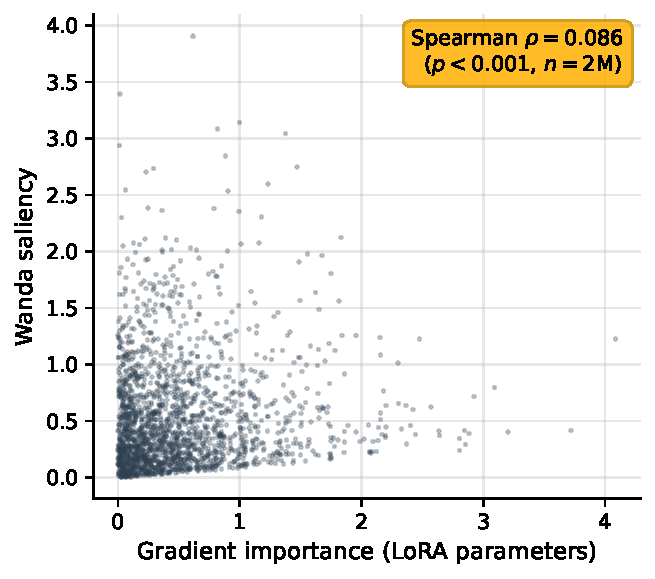
\includegraphics[width=0.45\textwidth]{figures/fig2_spearman.pdf}
\caption{Spearman $\rho = 0.086$ between Wanda and gradient importance (LoRA parameters) on Qwen2.5-3B. These metrics rank parameters nearly independently.}
\label{fig:spearman}
\end{figure}

Spearman correlation between Wanda ($|W| \times \text{RMS}(X)$) and gradient importance ($|\partial \mathcal{L}/\partial w|$) across 2M sampled parameters: (Figure~\ref{fig:spearman}; $\rho = 0.086$, 95\% CI $\approx [0.084, 0.088]$, $n{=}2$M; correlation-only, measured outside a continual-learning context).

\section{Confounded Null-Result Statistics}
\label{app:null_stats}

\begin{table}[h]
\caption{Per-seed BWT breakdown (Qwen2.5-3B, rank-16 LoRA, 5 tasks).}
\label{tab:per_seed}
\centering
\small
\begin{tabular}{@{}lccc@{}}
\toprule
\textbf{Seed} & \textbf{Gradient BWT $\downarrow$} & \textbf{Random BWT $\downarrow$} & \textbf{No Mask BWT $\downarrow$} \\
\midrule
42  & 0.491 & 0.435 & 0.507 \\
123 & 0.463 & 0.417 & $\mathbf{0.409}$ \\
456 & $\mathbf{0.388}$ & 0.414 & 0.539 \\
789 & $\mathbf{0.357}$ & 0.417 & 0.484 \\
1024 & 0.486 & 0.458 & 0.479 \\
\midrule
Mean & 0.437 & $\mathbf{0.428}$ & 0.484 \\
Std  & 0.061 & 0.019 & 0.047 \\
\bottomrule
\end{tabular}
\end{table}

\begin{table}[h]
\caption{Confounded comparison (Qwen2.5-3B, rank-16 LoRA, 5 tasks, $n{=}5$ seeds). The last column records whether an additional calibration forward--backward pass is required; its time and data costs are described in Appendix~\ref{app:attribution_cost}. Across all tables, bold marks the better value in its column.}
\label{tab:cl_3b}
\centering
\small
\begin{tabular}{@{}lccc@{}}
\toprule
\textbf{Method} & \textbf{BWT $\downarrow$} & \textbf{Loss $\downarrow$} & \textbf{Calibration pass?} \\
\midrule
Shared random & $\mathbf{0.428} \pm 0.019$ & $\mathbf{1.940} \pm 0.021$ & No \\
Gradient mask & $0.437 \pm 0.061$ & $1.966 \pm 0.037$ & Yes \\
No mask & $0.484 \pm 0.047$ & $1.970 \pm 0.033$ & No \\
\bottomrule
\end{tabular}
\end{table}


A paired $t$-test on per-seed BWT (Table~\ref{tab:per_seed}; random vs.\ gradient: seeds 42/123/456/789/1024 yield differences $+0.056$, $+0.046$, $-0.026$, $-0.059$, $+0.028$) gives $t(4) = 0.41$, $p = 0.70$ (two-tailed), Cohen's $d_z = 0.18$ (small effect). 
% With $n{=}5$ and observed $\text{SD}_\text{diff} = 0.049$, the minimum detectable BWT difference at $\alpha = 0.05$ is approximately 0.06 at 80\% power, larger than the observed mean difference of 0.009. 
The direction is seed-dependent, consistent with no systematic advantage for either method. Normalizing BWT per task by zero-shot loss ($\Delta L / L_0$) does not change the method ranking. Tables~\ref{tab:cl_3b} and~\ref{tab:within_b} report different \texttt{full\_alora} BWT for the same seed because they come from independent runs; the absolute BWT level varies across sessions (\S\ref{app:nf4_drift}).

% \section{Confounded Comparison Table}
% \label{app:confounded_table}

% Table~\ref{tab:cl_3b} gives the full confounded-design comparison discussed in \S\ref{sec:confounded}. The design varies pool and criterion together, so it is reported for completeness rather than as evidence about the selection rule.


\section{Within-\texttt{lora\_B} Comparison (Density-Unmatched)}
\label{app:within_b}

The within-\texttt{lora\_B} comparison matches the parameter pool (both arms draw from \texttt{lora\_B}) but \emph{not} the density: the gradient mask activates approximately $2\times$ the B parameters of random-B-only. It is therefore an intermediate, density-unmatched step; the density-matched control (D1) is the headline comparison in the main text. All comparisons are within-run (same method ordering and RNG state); $\Delta = \text{random\_B\_only} - \text{Grad-Full}$, negative $\Delta$ favors random-B. Absolute BWT values carry session-level variation and should not be compared across seeds (\S\ref{app:nf4_drift}).

\begin{table}[t]
\caption{Within-\texttt{lora\_B} comparison (Qwen2.5-3B, rank-16 LoRA, 5 tasks, 7 seeds). All comparisons are within-run (same method ordering and RNG state). $\Delta = \text{random\_B\_only} - \text{Grad-Full}$; negative $\Delta$ indicates random-B achieves lower (better) BWT.}
\label{tab:within_b}
\centering
\small
\begin{tabular}{@{}lccr@{}}
\toprule
\textbf{Seed} & \textbf{random\_B\_only BWT $\downarrow$} & \textbf{full\_alora BWT $\downarrow$} & \textbf{$\Delta$} \\
\midrule
42  & $\mathbf{0.326}$ & 0.491 & $-0.165$ \\
123 & $\mathbf{0.320}$ & 0.413 & $-0.093$ \\
456 & $\mathbf{0.337}$ & 0.356 & $-0.019$ \\
789 & $\mathbf{0.346}$ & 0.364 & $-0.018$ \\
1024 & $\mathbf{0.336}$ & 0.442 & $-0.106$ \\
2048 & $\mathbf{0.367}$ & 0.402 & $-0.035$ \\
4096 & $\mathbf{0.331}$ & 0.398 & $-0.067$ \\
\midrule
Mean & $\mathbf{0.338} \pm 0.015$ & $0.409 \pm 0.046$ & $-0.072$ \\
\bottomrule
\end{tabular}
\end{table}

\section{Variation Across Runs and Method-Order Variation}
\label{app:nf4_drift}

Three quantities in this paper are sometimes read as competing estimates of one
noise level. They are not: each measures a different thing at a different
granularity, and the table below separates them.

\begin{table}[h]
\caption{Distinct quantities that are sometimes all called run-to-run \emph{noise}. The paired tests use the across-seed SD of the within-session contrasts; the protocol-equivalence discrepancy is an implementation check and does not enter inference. Position and cross-session effects are reported as sensitivities rather than as interchangeable error estimates.}
\label{tab:noise_levels}
\centering
\small
\begin{tabular}{@{}p{0.17\textwidth}p{0.17\textwidth}p{0.16\textwidth}p{0.38\textwidth}@{}}
\toprule
\textbf{Level} & \textbf{What varies} & \textbf{Magnitude} & \textbf{What it measures} \\
\midrule
(a) protocol-equivalence check & execution path only & $9.6 \times 10^{-5}$ & numerical agreement between two code paths; not an inferential error term \\
(b) across-seed paired contrast & independent seed & SD$(\Delta_s)=0.071$ & variability used by the paired significance test \\
(c) position (ordering) sensitivity & position of the two arms & $0.064$ (seed 42, \texttt{gradient\_B}) & method-position interaction in a three-seed check \\
(d) cross-session variation & session, hardware, and method & up to $0.120$ (\texttt{full\_alora}, seed 42) & method-specific offset of unknown origin \\
\bottomrule
\end{tabular}
\end{table}

\begin{table}[h]
\caption{Method-ordering sensitivity (D1 density-matched, three seeds). $\Delta_{\text{pos}}$ is the BWT difference between running at position~1 and position~2. The last two columns express each arm's positional shift as a fraction of the main D1 contrast ($|\Delta| = 0.155$).}
\label{tab:method_order}
\centering
\small
\begin{tabular}{@{}lccrr@{}}
\toprule
\textbf{Seed} & $|\Delta_{\text{pos}}(\text{rB})|$ & $|\Delta_{\text{pos}}(\text{gB})|$ & \textbf{rB / main} & \textbf{gB / main} \\
\midrule
42   & $1.5 \times 10^{-3}$ & $6.4 \times 10^{-2}$ & 0.01 & 0.41 \\
789  & $3.1 \times 10^{-5}$ & $6.2 \times 10^{-3}$ & 0.00 & 0.04 \\
2048 & $8.4 \times 10^{-6}$ & $1.3 \times 10^{-2}$ & 0.00 & 0.08 \\
\bottomrule
\end{tabular}
\end{table}

\paragraph{(a) Same process, protocol split.} Running each method in its own
process reproduces the multi-method BWT to within $9.6\times10^{-5}$, an order of
magnitude below the pre-specified $10^{-3}$ threshold. This is a check on the
protocol implementation, not on run-to-run variation of the model: two code
paths that should agree do agree. The paired $t$ tests instead use the
across-seed standard deviation of the within-session paired contrasts,
SD$(\Delta_s)=0.071$ for D1.

\paragraph{(b) Same session, arm order swapped.} Within one D1 session the two
arms run back to back, and reversing their order is a genuine perturbation of
the run. At seed 42 the \texttt{gradient\_B} arm's BWT moves by 0.064 between the
two orders; at seeds 789 and 2048 both arms
stay within $1.4\times10^{-2}$. This is a within-session positional effect, and
the within-run contrast survives it at all three tested seeds. Because this
sensitivity analysis covers three rather than seven seeds, it does not establish
the population distribution of the position effect.

\paragraph{(c) Cross-session, same seed.} The absolute BWT of a fixed method and
seed is not reproducible across sessions. For seed 42, \texttt{full\_alora}
records $0.491$, $0.378$, and $0.498$ in three separate runs (spread $0.120$),
while \texttt{random\_B\_only} records $0.326$, $0.324$, and $0.278$ (spread
$0.048$). The spread is method-dependent, so it does not act as a constant offset
that cancels in a comparison.

Method position can shift the absolute BWT of Gradient-B, most notably at seed 42, but reversing the execution order does not reverse the Random-B–Grad-B contrast in any of the three tested seeds. (Table~\ref{tab:method_order})

\begin{table}[h]
\caption{Absolute loss-based BWT for the same seed 42 under identical method
definitions, across sessions and hardware. Run C is the D1 density-matched
session and Run D the uniform-B suppression control (the M2 controller) session, both on a separate GPU and software
stack; \texttt{random\_A+B} was not run in either. A Run-D entry exists only for
methods Run D ran, and it did not train a plain \texttt{full\_alora} arm, so that
cell is \texttt{---} and its gradient-side arm is \texttt{gradient\_B}, entered on
its own row. Spread is $\max-\min$ across the runs in which the method appears.}
\label{tab:nf4_drift}
\centering
\small
\begin{tabular}{@{}lcccc@{}}
\toprule
\textbf{Method} & \textbf{Run A} & \textbf{Run B} & \textbf{Run C} & \textbf{Run D / spread} \\
\midrule
Gradient mask (\texttt{full\_alora}) & 0.491 & 0.378 & 0.498 & --- (0.120) \\
Gradient-B@10\% (\texttt{gradient\_B}) & --- & --- & 0.453 & 0.423 (0.030) \\
Random mask (\texttt{random\_A+B}) & 0.435 & 0.349 & --- & --- \\
Random B-only (\texttt{random\_B\_only}) & 0.326 & 0.324 & 0.278 & 0.278 (0.048) \\
\bottomrule
\end{tabular}
\end{table}

\paragraph{Why this is not called NF4 non-determinism.} Quantization is the same
in every run of Table~\ref{tab:nf4_drift}, so it cannot by itself explain a
cross-session spread while leaving a same-process protocol split at
$9.6\times10^{-5}$. The cross-session spread is method-specific rather than a
common shift shared by all arms. We therefore report it as a \emph{method-specific
cross-session offset of unknown origin} and do not
attribute it to a mechanism. Two consequences follow. First, only within-run
comparisons are used for any claim in this paper. Second, the \texttt{random\_B\_only}
value that enters Table~\ref{tab:d1} is the D1 session's own $0.278$, taken from the
same session as its partner arm, not an average across sessions.

\paragraph{Attribution of the level (c) spread.} The level (c) spread has no single
cause. Method position is not such a cause within a session:
\texttt{set\_seed} is called before each method's model load and no random numbers
are consumed between iterations, so the seed state entering training does not
depend on position. Level (b) shows that position can still matter, and level
(c) shows that session identity can. Which of these dominates across a full
re-run is not tested here.

Therefore, absolute BWT levels should not be compared across sessions; all statistical claims in the paper use within-session paired contrasts.

\section{RRM Boundary Analysis}
\label{app:rrm}

We investigated whether assigning each task a different random mask (Rotating Random Masks, RRM) provides additional benefit beyond shared random masking. RRM generates a deterministic per-task mask via $m^{(t)}_i = \mathbf{1}[\text{hash}(t \| i) \bmod 10 < k]$, reducing expected pairwise inter-task parameter overlap from 100\% (shared mask) to $k^2$ (1\% at 10\% sparsity) (Table~\ref{tab:rrm_boundary} ). 
% reports RRM versus shared random across LoRA ranks and task order.

\begin{table}[h]
\caption{RRM boundary analysis (Qwen2.5-3B, single seed per condition except rank-16 reference).}
\label{tab:rrm_boundary}
\centering
\small
\begin{tabular}{@{}lccrl@{}}
\toprule
\textbf{Condition} & \textbf{RRM BWT} & \textbf{Random BWT} & \textbf{$\Delta$} & \textbf{Direction} \\
\midrule
Rank 4 & 0.464 & 0.423 & $+$0.041 & Random better \\
Rank 8 & 0.427 & 0.373 & $+$0.055 & Random better \\
Rank 16 (ref.) & 0.401 & 0.435 & $-$0.034 & RRM better \\
Rank 32 & 0.414 & 0.390 & $+$0.024 & Random better \\
Reverse order & 0.115 & 0.109 & $+$0.006 & Random better \\
\bottomrule
\end{tabular}
\end{table}

RRM shows a favorable paired difference at rank 16 only. The overlap-reduction hypothesis predicts a consistent RRM advantage; the data do not support this across conditions. RRM's effect appears condition-dependent rather than robust.

\section{Sparsity Sweep}
\label{app:sparsity}

We sweep the masking budget over 5\%, 10\%, 20\%, and 30\% (single seed) to test whether the within-pool ordering is specific to the 10\% sparsity used in the main experiments. Across all four levels, shared random achieves numerically lower BWT than gradient attribution, with no cross-over; the largest margin is at 30\%.

\begin{figure}[ht]
\centering
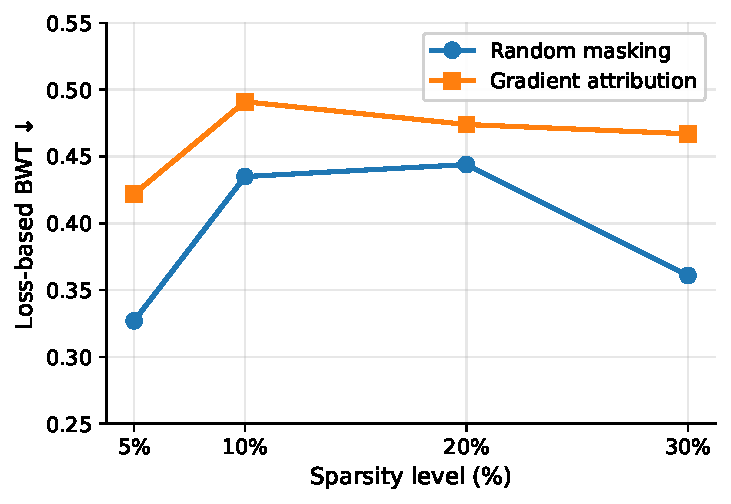
\includegraphics[width=0.55\textwidth]{figures/fig3_sparsity.pdf}
\caption{Sparsity sweep (Qwen2.5-3B, single seed). Shared random achieves numerically lower BWT than gradient attribution at all four tested levels.}
\label{fig:sparsity}
\end{figure}

\begin{table}[h]
\caption{Sparsity sweep numerical values (Qwen2.5-3B, single seed). Random BWT $\leq$ Gradient BWT at all tested levels.}
\label{tab:sparsity}
\centering
\small
\begin{tabular}{@{}lcc@{}}
\toprule
\textbf{Sparsity} & \textbf{Random BWT $\downarrow$} & \textbf{Gradient BWT $\downarrow$} \\
\midrule
5\% & 0.327 & 0.422 \\
10\% & 0.435 & 0.491 \\
20\% & 0.444 & 0.474 \\
30\% & 0.361 & 0.467 \\
\bottomrule
\end{tabular}
\end{table}

\section{Training Stability: Rank-8 No-Mask Divergence}
\label{app:training_stability}

The rank-8 no-mask ablation reveals a discrepancy between two endpoint-based forgetting summaries. Endpoint BWT is 0.176; average forgetting is 0.2837. Training produced a severe loss spike during task 4 (Math): evaluation losses on three prior tasks exceeded 14, compared to values below 4 for all masked conditions at the same rank. This spike subsequently recovered during task 5, yielding deceptively low endpoint BWT. We do not interpret the rank-8 no-mask endpoint BWT of 0.176 as evidence that no-mask outperforms masking.

The same signature recurs at rank 16 and is seed-dependent: at seed 123 the unmasked arm spiked during task 4 with evaluation losses of 16.2/16.0/14.7 on the three prior tasks (code/medical/legal), while every masked arm in that run stayed below $2.5$; at seed 42 the unmasked arm did \emph{not} spike (task-4 evaluations $\leq 1.2$). The instability is therefore a property of the unmasked (all-parameter) configuration rather than of a particular rank, and it appears in a minority of seeds.

\section{Mask Concentration by Module}
\label{app:mask_concentration}

The o\_proj suppression ablation and module-concentration figures, discussed in \S\ref{sec:analysis}, are reproduced below together with the module-concentration table for reference.

\begin{figure}[t]
\centering
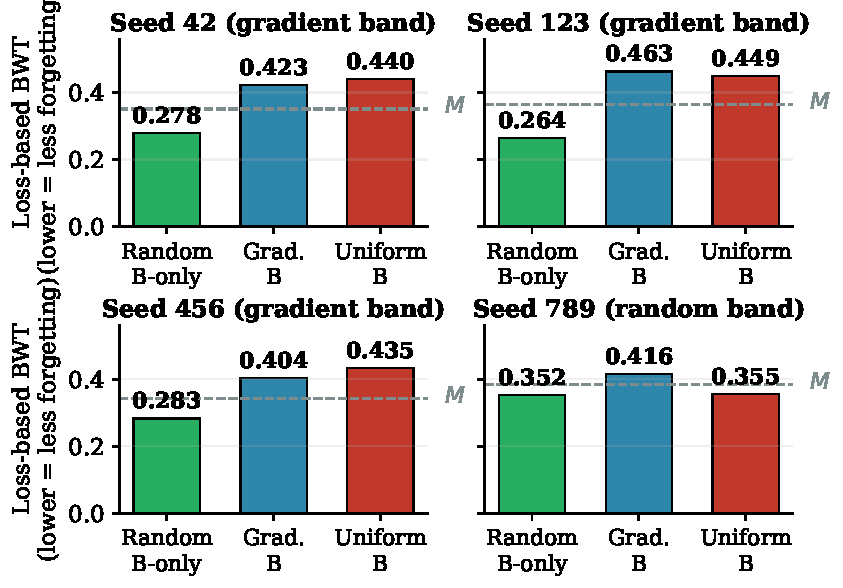
\includegraphics[width=0.6\textwidth]{figures/fig_oproj_ablation.pdf}
\caption{The suppression control's outcome is \emph{seed-dependent}. All three arms train 1{,}651{,}508 parameters, which is 5.5\% of the full LoRA pool (each arm draws 10\% of the \texttt{lora\_B} sub-pool, and $B$ holds 55\% of the pool's parameters), so this is the density-matched setting throughout. The uniform-B controller redistributes the gradient mask's budget uniformly across LoRA modules. At seed 42 it sits in the gradient band (0.440 above gradient-B's 0.423 and well above random-B-only's 0.278); seeds 123 and 456 also land on the gradient side; at seed 789 it falls to the random band (0.355 below gradient-B's 0.416, alongside random-B-only's 0.352). Three of four seeds fall on the gradient side. M2 is an independent session from D1, so the same-seed gradient-B values differ between them (e.g.\ seed 42: 0.423 here vs 0.453 in the D1 table; seed 789: 0.416 vs 0.387; \S\ref{app:nf4_drift}). We therefore do not treat this ablation as establishing the \texttt{o\_proj}-concentration mechanism (\S\ref{sec:analysis}).}
\label{fig:oproj_ablation_main}
\end{figure}

\begin{figure}[t]
\centering
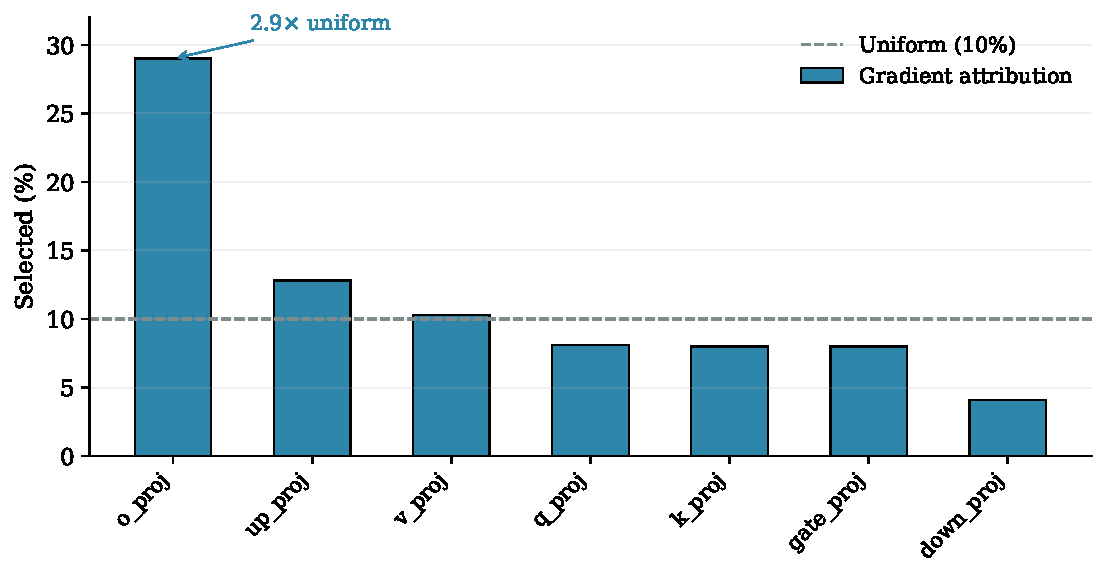
\includegraphics[width=0.5\textwidth]{figures/fig_module_concentration.pdf}
\caption{Gradient-mask concentration by LoRA module (Qwen2.5-3B). Gradient attribution selects 29\% of \texttt{o\_proj} parameters (2.9$\times$ the 10\% uniform rate) and is under-represented in \texttt{down\_proj} (4.1\%); the dashed line marks uniform 10\% selection.}
\label{fig:module_concentration_main}
\end{figure}

\begin{table}[t]
\caption{Gradient mask concentration by LoRA module (Qwen2.5-3B). Random masking distributes uniformly at 10\% per module. Gradient attribution selects exclusively \texttt{lora\_B} parameters (all \texttt{lora\_A} receive zero importance due to $B=0$ initialization).}
\label{tab:mask_concentration}
\centering
\small
\begin{tabular}{@{}lccr@{}}
\toprule
\textbf{Module} & \textbf{Gradient density} & \textbf{Random density} & \textbf{Ratio} \\
\midrule
o\_proj & 29.0\% & 10.0\% & 2.9$\times$ \\
up\_proj & 12.8\% & 10.0\% & 1.3$\times$ \\
v\_proj & 10.3\% & 10.0\% & 1.0$\times$ \\
q\_proj & 8.1\% & 10.0\% & 0.8$\times$ \\
k\_proj & 8.0\% & 10.0\% & 0.8$\times$ \\
gate\_proj & 8.0\% & 10.0\% & 0.8$\times$ \\
down\_proj & 4.1\% & 10.0\% & 0.4$\times$ \\
\bottomrule
\end{tabular}
\end{table}


\section{Generalization and Boundary Checks}
\paragraph{Scale Observations}
\label{app:scale}

We additionally observe the within-pool comparison at three parameter scales (0.5B, 1.5B, 7B; single seed each). These are observational rather than multi-seed, and at 0.5B and 1.5B only the shared-random and no-mask conditions were run, so no gradient attribution baseline is available for a direct comparison there.

\begin{table}[ht]
\caption{BWT at additional scales (single seed, observational).}
\label{tab:scale_obs}
\centering
\small
\begin{tabular}{@{}lccc@{}}
\toprule
\textbf{Scale} & \textbf{Random BWT $\downarrow$} & \textbf{Gradient BWT $\downarrow$} & \textbf{No Mask BWT $\downarrow$} \\
\midrule
0.5B & 0.343 & --- & 0.431 \\
1.5B & 0.309 & --- & 0.356 \\
7B & 0.447 & 0.441 & 0.514 \\
\bottomrule
\end{tabular}
\end{table}


\paragraph{Task Ordering (single seed)}
\label{app:task_order}

A reversed-order experiment yields BWT $\approx 0.11$ for all masking methods, compared to $\approx 0.42$ under the standard order, a nearly $4{\times}$ reduction that far exceeds the method differences measured within this experiment (within-session method contrasts of order $10^{-2}$). This is a \emph{single seed}, so the $4{\times}$ magnitude is a qualitative pointer, not a quantitative estimate; it is reported to show that task ordering dominates the forgetting landscape, not as a measured effect size. The conclusions of this paper apply only to the tested Code$\to$Medical$\to$Legal$\to$Math$\to$Creative sequence; additional task orderings with multi-seed replication are needed before the null result can be generalized.

\paragraph{Cross-Architecture Comparison}
\label{app:cross_arch}

Both cross-architecture designs are tabulated in Table~\ref{tab:cross_arch}: the confounded design (gradient selecting B-only, random selecting A+B) and the within-\texttt{lora\_B} design (both methods restricted to \texttt{lora\_B}). The two designs are not comparable row-for-row because the Phi-2 within-B rows use a different LoRA target set; \S\ref{sec:boundaries} discusses both.

\begin{table}[t]
\caption{Cross-architecture comparison on Qwen2.5-3B and Phi-2 (2.78B, GPT-NeoX-style), with both arms within a row sharing one target set. Qwen2.5-3B targets \texttt{q/k/v/o/gate/up/down\_proj} (pool $29{,}933{,}568$), whereas Phi-2 uses GPT-NeoX-style \texttt{q,k,v,fc1,fc2,dense} projections (pool $23{,}592{,}960$) in the confounded design. In the within-\texttt{lora\_B} design, the Phi-2 rows omit \texttt{dense} (pool $20{,}971{,}520$, 12.5\% smaller), so the two Phi-2 designs are not comparable row-for-row. The within-\texttt{lora\_B} rows are matched on pool but \emph{not} density (the gradient mask activates approximately $2\times$ the B parameters of Random-B), as on Qwen2.5-3B.}
\label{tab:cross_arch}
\centering
\small
\begin{tabular}{@{}llccc@{}}
\toprule
\textbf{Architecture} & \textbf{Comparison} & \textbf{Grad.\ BWT $\downarrow$} & \textbf{Rand.\ BWT $\downarrow$} & \textbf{$\Delta$} \\
\midrule
Qwen2.5-3B ($n{=}5$) & Confounded & $0.437 \pm 0.061$ & $0.428 \pm 0.019$ & $-0.009$ \\
Phi-2 ($n{=}5$) & Confounded & $0.158 \pm 0.019$ & $0.183 \pm 0.016$ & $+0.025$ \\
\midrule
Qwen2.5-3B ($n{=}7$) & Within-B & $0.409 \pm 0.046$ & $0.338 \pm 0.015$ & $-0.072$ \\
Phi-2 ($n{=}4$) & Within-B & $0.149 \pm 0.036$ & $0.065 \pm 0.017$ & $-0.084$ \\
\bottomrule
\end{tabular}
\end{table} 
% \section{Method Ordering Within a D1 Session (three seeds)}
% \label{app:method_order}

% The D1 density-matched control runs two arms sequentially in one process: \texttt{random\_B\_only} then \texttt{gradient\_B} (Run~A), or the reverse (Run~B). If method position within a session affects BWT, the within-run contrast ($\text{random\_B\_only} - \text{gradient\_B}$) would change sign or magnitude when the order is reversed. We test this at three seeds (42, 789, 2048).

% \paragraph{Design.} Each seed produces two independent processes sharing the same model weights, LoRA configuration, and mask; only the execution order of the two arms differs. We report $\Delta_{\text{pos}}(\text{arm}) = \text{BWT}(\text{arm, position 1}) - \text{BWT}(\text{arm, position 2})$ for each arm and each seed.

% \paragraph{Results.}


% Table~\ref{tab:method_order} reports all three seeds. For the \texttt{random\_B\_only} arm the positional shift is negligible everywhere, at most $1.5\times10^{-3}$, which is one hundredth of the main contrast. For the \texttt{gradient\_B} arm the shift is larger and seed-dependent: 0.064 at seed 42, which is 41\% of the main contrast, but only 0.006 and 0.013 at seeds 789 and 2048, or 4\% and 8\% of it. Position therefore matters for one arm at one seed, and is otherwise small against the effect being measured.

% \paragraph{Interpretation.} These are three individual observations, not a distribution. At seed~42 the two readings remain open and inseparable at $n{=}1$: the $\Delta_{\text{pos}}$ values are either a real position effect or an artifact of treating a position offset as if it were the paired-comparison error, and the two later seeds favour the second reading. At seed~789 both arms recorded higher BWT at position~2 ($\Delta_{\text{pos}}$ negative for \texttt{gradient\_B}), so a session-level shift is not excluded for that seed. At seed~2048 the arms moved in opposite directions, ruling out a pure session shift there.

% The within-run contrast ($\text{random\_B\_only} - \text{gradient\_B}$) is negative under both orders at all three seeds (seed~42: Run~A $= -0.121$, Run~B $= -0.186$; seed~2048: Run~A $= -0.257$, Run~B $= -0.270$), so the D1 direction survives order reversal.

\section{In-Domain Calibration Ablation}
\label{app:calibration}

The primary experiments use out-of-domain Alpaca calibration data (64 samples). To test whether this choice drives the null result, we repeat the gradient-mask experiment with \emph{pooled in-domain} calibration: 60 samples drawn equally from the five CL tasks.\footnote{$\lfloor 64/5 \rfloor \times 5 = 60$; a 6.25\% size difference from integer division.} All other parameters are identical (Qwen2.5-3B, seed 42, rank 16, 10\% sparsity).

Loss-based BWT is 0.495 vs 0.491 with Alpaca calibration ($\Delta = 0.004$, 0.8\% relative), well within the 5-seed standard deviation of 0.061. Random and no-mask controls are numerically identical across both runs, confirming infrastructure determinism. The \emph{cross-calibration} overlap (Alpaca vs pooled) is Jaccard $= 0.585$: changing the calibration domain alters 42\% of selected parameters. Despite this substantial mask difference, BWT changes by only 0.004. This robustness is of the \emph{outcome}, not the mask: the mask does change, but \emph{among gradient-derived masks} the specific 10\% selected has little influence on forgetting, whereas swapping the selection criterion entirely (gradient for random) does, as the density-matched control shows (\S\ref{sec:confounded}).

\section{B=0 Restriction Asymmetry}
\label{app:b0_asymmetry}

The within-\texttt{lora\_B} comparison varies the selection criterion while holding the parameter pool fixed. That the pool restriction is the right control to hold follows from an asymmetry between the two arms at seed 42 (Table~\ref{tab:b0_asymmetry}). Restricting the gradient mask to \texttt{lora\_B} changes nothing, because under $B=0$ every \texttt{lora\_A} importance score is already zero and the restriction is a no-op. The same restriction applied to the random arm removes the \texttt{lora\_A} dilution and improves BWT by 0.025. A restriction that does nothing to one arm and helps the other is evidence that the two arms were drawing from different pools before the restriction was applied, which is what makes the pool-matched comparison the informative one.

\begin{table}[h]
\centering\small
\caption{Effect of restricting the mask to \texttt{lora\_B} (seed 42). For gradient attribution, the restriction is a no-op by construction (B=0 collapses every \texttt{lora\_A} importance score to zero); for random, restricting to B removes \texttt{lora\_A} dilution and improves BWT by 0.025. This asymmetry demonstrates that the within-B comparison varies the selection criterion, not the parameter pool.}
\label{tab:b0_asymmetry}
\begin{tabular}{@{}lccc@{}}
\toprule
\textbf{Method} & \textbf{Unrestricted BWT} & \textbf{B-only BWT} & \textbf{Gap} \\
\midrule
Gradient & 0.378 & 0.378 & $+0.000$ \\
Random   & 0.349 & 0.324 & $-0.025$ \\
\bottomrule
\end{tabular}
\end{table}


\section{Per-Seed Accuracy and Matched Loss Contrast}
\label{app:accuracy_seeds}

The accuracy evaluation is reported in the main text, \S\ref{sec:accuracy_branch}, together with the option-scoring protocol; its per-seed values and the matched loss contrast are tabulated below. (Table~\ref{tab:accuracy_branch})

\begin{table}[t]
\caption{Per-seed results, with both columns reported under the sign convention [Grad $-$ Random]. Col.~2 is the accuracy-BWT difference: the difference in mean final-minus-learned option-scoring accuracy over the prior discrete-option tasks (Medical and Legal), not a difference of final accuracies. It is therefore a retention quantity on the same footing as the loss-based BWT column. Col.~2 is reported in percentage points in every row and carries the 95\% $t$-interval on the seven-seed mean. Col.~3 is the loss-based BWT difference on the same A800 environment and has mean $+0.152$ (SD $0.0749$, $t = 5.37$, CI $[+0.083, +0.221]$, 7/7 same direction). The V100 contrast is $+0.155$ under the same [Grad $-$ Random] convention. Across matched seeds, the A800-minus-V100 contrast difference has mean $-0.0033$ and SD $0.0441$, so replication is strongest at the mean and directional levels rather than as seed-wise numerical identity.}
\label{tab:accuracy_branch}
\centering
\small
\begin{tabular}{@{}lrr@{}}
\toprule
\textbf{Seed} & \textbf{Accuracy-BWT $\Delta$ [Grad $-$ Rand], pp} & \textbf{Loss BWT $\Delta$ [Grad $-$ Rand]} \\
\midrule
42   & $+2.00$ & $+0.2320$ \\
123  & $0.00$  & $+0.1647$ \\
456  & $+0.48$ & $+0.1300$ \\
789  & $-6.98$ & $+0.0786$ \\
1024 & $+4.60$ & $+0.0514$ \\
2048 & $+0.51$ & $+0.2572$ \\
4096 & $+6.00$ & $+0.1492$ \\
\midrule
\multicolumn{3}{@{}l}{\emph{Summary (column 2 in percentage points, column 3 in BWT units)}} \\
Mean & $+0.94$\,pp & $+0.152$ \\
SD   & $4.17$\,pp & $0.0749$ \\
95\% CI & $[-2.91, +4.80]$\,pp & $[+0.083, +0.221]$ \\
\bottomrule
\end{tabular}
\end{table}


\section{The Math Task: Truncation Audit}
\label{app:math_audit}

Loss on math decreases with training while accuracy on the same task collapses to zero for all arms: peak accuracy at math's own training phase is $0.04$ and every arm ends at $0.00$. The numeric-match function accepts a bare number, a number with surrounding text, and a complete solution, and the prompt prefixes are identical; nevertheless, the interaction between output format and the 256-token limit makes the generation-based score unreliable. A generation audit reports 56--95\% of generations across all tasks and arms reaching the cap without an end-of-sequence token, and for math specifically 81--90\% of generations reach the cap. The last number in a truncated solution is often an intermediate quantity, so the reference answer is absent from the value the scorer inspects. Every arm shares the same cap and scorer, so the bias is common rather than arm-specific. We do not treat the math column as a forgetting result: under option-based scoring math yields no score, and under generation scoring it is confounded with truncation.

% \section{Limitations}
% \label{app:limitations}


% \begin{itemize}[leftmargin=*,itemsep=2pt,topsep=2pt]
% \item \emph{Static masks only.} All methods reuse a single static mask across all five tasks. Whether adaptive per-task gradient masks (recomputed after each task's training) would change the outcome remains an open question; this is the broadest scope limitation of the present study.
% \item \emph{Absolute BWT is not reproducible across sessions.} The same method and seed produces absolute BWT values that vary by up to $\sim$0.12 between sessions, a spread that approaches the within-B advantage ($\Delta = 0.072$). This is not a random perturbation of a comparison and we do not attribute it to a mechanism; it is a property of the absolute level a session settles at (Appendix~\ref{app:nf4_drift} separates this from two other, smaller run-to-run quantities). The consequence is scope, not invalidity: \emph{only within-run comparisons are valid}, and every method comparison in this paper is within-run, sharing one RNG state and one method ordering.
% \item \emph{B-pool advantage is not robust.} Restricting the random mask to the \texttt{lora\_B} pool (\texttt{random\_B\_only}) does not consistently outperform the unrestricted random mask (\texttt{random\_A+B}); the direction is seed-dependent and the mean difference is small relative to the cross-session spread, so this is not a systematic effect. The pool restriction therefore acts as a supporting observation in this paper; the density-matched comparison carries the headline claim.\footnote{Within-B vs gradient attribution is the headline (7/7 consistent, $p = 0.012$); within-B vs random-A+B is seed-dependent.}
% \item \emph{Loss-based evaluation with an accuracy consistency check.} All multi-seed statistical tests are loss-based BWT. An accuracy evaluation over the same seven seeds, on the two discrete-option tasks (Medical and Legal, 100 items each), returns a mean gradient-minus-random difference of $+0.94$ percentage points with a 95\% interval of $[-2.91, +4.80]$ percentage points. The two masks are indistinguishable on accuracy. A 4-percentage-point non-inferiority margin was specified in advance for this interval and is not met (upper bound $+4.80$ percentage points). Accuracy differences of up to about 4.8 percentage points in the gradient mask's favour are not excluded by this measurement. See \S\ref{sec:accuracy_branch}. Conclusions are scoped to the loss metric for all multi-seed claims.
% \item \emph{Calibration domain tested but not exhaustively.} A pooled in-domain calibration ablation (single seed) changed 42\% of selected parameters yet produced near-identical BWT ($\Delta = 0.004$; \S\ref{app:calibration}). The remaining untested variant is per-task calibration (a separate mask per task).
% \item \emph{Single task order.} The fixed Code$\to$Medical$\to$Legal$\to$Math$\to$Creative order is the primary condition. A reversed-order experiment (single seed) yields BWT $\approx 0.11$ for all methods, a nearly $4{\times}$ reduction; conclusions are specific to the tested sequence.
% \item \emph{Statistical power ($n{=}7$).} With seven seeds the within-B comparison is significant on both parametric and non-parametric tests (paired $t(6) = -3.53$, $p = 0.012$; Wilcoxon $p = 0.016$), with 7/7 seeds directionally consistent and a large effect size ($d_z = -1.34$). The 7-seed paired test uses within-run differences, which are unaffected by the cross-session spread; the reported means ($0.338$ vs $0.409$) are cross-session averages and carry $\pm 0.12$ uncertainty.
% \item \emph{Single LoRA rank.} Multi-seed results are at rank 16 only; other ranks are single-seed.
% \item \emph{Zero-init LoRA only.} The B=0 mechanism and within-B comparison apply only to standard zero-init LoRA. PiSSA~\citep{meng2024pissa} and other non-zero initialization variants are not tested.
% \end{itemize}

\section{Positioning Against Gradient-Attribution Families}
\label{app:positioning}

Table~\ref{tab:positioning} places our contribution against the gradient-attribution families we are positioned against, on the two axes that drive the study.

\begin{table}[h]
\centering
\small
\caption{Positioning against gradient-attribution families. "B=0 pool" isolates the \texttt{lora\_B} pool; "within-pool grad-vs-random" compares gradient to a matched random baseline in a shared pool.}
\label{tab:positioning}
\begin{tabular}{@{}lcc@{}}
\toprule
\textbf{Method} & \textbf{B=0 pool} & \textbf{Within-pool grad-vs-random} \\
\midrule
EWC / SI / MAS & No & No \\
PiSSA ($B\neq0$) & N/A by init & No \\
Attribution-Guided CL & Unclear$^{\dagger}$ & Unclear$^{\dagger}$ \\
\textbf{Ours (within-\texttt{lora\_B})} & \textbf{Yes} & \textbf{Yes} \\
\bottomrule
\end{tabular}
\parbox{0.88\textwidth}{\footnotesize $^{\dagger}$The published description does not establish all initialization, attribution-timing, baseline-pool, and mask-scope details required to classify these two axes; we therefore do not infer a pool mismatch.}
\end{table}

Table~\ref{tab:rule_positioning} lists the selection rules this paper is positioned against and marks which we train under one protocol. Only the rules we train contribute empirical numbers here; the rest are compared by their published design, with none of their reported numbers presented as a measurement of ours.

\begin{table}[h]
\centering
\footnotesize
\caption{Selection rules this paper is positioned against. The last column marks the four rules we train and evaluate under one protocol (\S\ref{sec:mask}); the rest are compared by design only, and none of their published numbers is cited as a result of ours.}
\label{tab:rule_positioning}
\begin{tabular}{@{}p{0.21\textwidth}p{0.59\textwidth}c@{}}
\toprule
\textbf{Rule} & \textbf{What it scores, and what for} & \textbf{Run} \\
\midrule
EWC~\citep{kirkpatrick2017overcoming}; MAS~\citep{aljundi2018memory} & Fisher information, output sensitivity; a penalty, not a mask & no \\
SNIP~\citep{lee2019snip}; GraSP~\citep{wang2020grasp} & gradient at initialisation; one-shot pruning mask & no \\
Wanda~\citep{sun2024wanda} & weight$\times$activation magnitude; one-shot pruning mask & no \\
LoRA-FA~\citep{zhang2023lorafa} & none, structural; freezes \texttt{lora\_A}, trains \texttt{lora\_B} & no \\
Grad-Full, Grad-B (\S\ref{sec:mask}) & calibration gradient magnitude; static CL mask, full pool (Grad-Full) or \texttt{lora\_B} at 10\% (Grad-B) & \textbf{yes} \\
Random-B; Random A+B~\citep{su2024random} & none, uniform; static CL mask, \texttt{lora\_B} at 10\% (Random-B) or full pool (A+B) & \textbf{yes} \\
\bottomrule
\end{tabular}
\end{table}

\section{D1 Per-Task and Per-Seed Decomposition}
\label{app:d1_per_task}

Table~\ref{tab:d1_per_task} gives the seven-seed mean per-task
contribution. Table~\ref{tab:d1_per_task_seeds} gives the same quantity for each
seed, so the task-level pattern can be checked against the seed-level one; the
main text reports the same decomposition as a figure (Figure~\ref{fig:per_task}). Each
entry is $\text{loss\_matrix}[4][j] - \text{loss\_matrix}[j][j]$ for prior task
$j$; the final column is the mean over the four tasks, which is the per-seed
aggregate $\Delta$ of Table~\ref{tab:d1}.

\begin{table}[!htbp]
\caption{D1 per-task decomposition of loss-based BWT, averaged over the seven seeds. Each entry is $\text{loss\_matrix}[4][j] - \text{loss\_matrix}[j][j]$ for prior task $j$, that task's contribution to the aggregate; the last column is its share of the aggregate $\Delta$ in absolute value. Creative is the final task and contributes no forgetting term. The aggregate is concentrated on medical (79.9\%) but not confined there: excluding medical the matched contrast remains $-0.042$ (7/7 negative), while code and math are each negative in 7/7 seeds and legal is not established.}
\label{tab:d1_per_task}
\centering
\small
\begin{tabular}{@{}lrrrr@{}}
\toprule
\textbf{Prior task} & \textbf{random-B} & \textbf{gradient-B} & \textbf{$\Delta$} & \textbf{share of $\Delta$} \\
\midrule
Code    & $-0.021$ & $0.025$ & $-0.046$ & 7.4\% \\
Medical & $0.998$ & $1.493$ & $-0.496$ & 79.9\% \\
Legal   & $0.007$ & $0.010$ & $-0.003$ & 0.5\% \\
Math    & $0.191$ & $0.266$ & $-0.076$ & 12.2\% \\
\midrule
Aggregate & $0.294$ & $0.449$ & $-0.155$ & 100\% \\
\bottomrule
\end{tabular}
\end{table}

\begin{table}[h]
\caption{Per-seed, per-task D1 decomposition ($\Delta = \text{random-B} - \text{gradient-B}$ for each prior task). Negative favours random-B. Legal is the only task whose sign is not consistent across seeds.}
\label{tab:d1_per_task_seeds}
\centering
\small
\begin{tabular}{@{}lrrrrr@{}}
\toprule
\textbf{Seed} & \textbf{Code} & \textbf{Medical} & \textbf{Legal} & \textbf{Math} & \textbf{Aggregate} \\
\midrule
42   & $-0.040$ & $-0.409$ & $-0.002$ & $-0.249$ & $-0.175$ \\
123  & $-0.002$ & $-0.698$ & $-0.002$ & $-0.052$ & $-0.188$ \\
456  & $-0.074$ & $-0.381$ & $-0.004$ & $-0.033$ & $-0.123$ \\
789  & $-0.063$ & $-0.054$ & $+0.001$ & $-0.023$ & $-0.035$ \\
1024 & $-0.044$ & $-0.410$ & $-0.011$ & $-0.021$ & $-0.121$ \\
2048 & $-0.041$ & $-0.950$ & $+0.010$ & $-0.062$ & $-0.261$ \\
4096 & $-0.059$ & $-0.568$ & $-0.014$ & $-0.091$ & $-0.183$ \\
\midrule
Mean & $-0.046$ & $-0.496$ & $-0.003$ & $-0.076$ & $-0.155$ \\
\bottomrule
\end{tabular}
\end{table}

\section{Ruling Out a Learning Deficit in the D1 Gap}
\label{app:d1_diagonal}

The D1 density-matched comparison (both arms 10\% of \texttt{lora\_B}, 1{,}651{,}508 parameters) shows random-B-only achieving lower BWT than gradient-B. One rival reading is that gradient-B's top-10\% is the more concentrated half of the original 20\% mask, so gradient-B learns each task less well and the gap is a learning deficit rather than a retention difference. The per-task diagonal losses (each task's loss immediately after it is learned) exclude this: gradient-B's diagonal loss is lower than random-B-only's in \emph{all} 35 seed$\times$task cells (7 seeds $\times$ 5 tasks), with no exceptions.

\begin{table}[ht]
\caption{Diagonal loss (mean $\pm$ std over the seven D1 seeds), by task. Lower is better. gradient-B is lower than random-B-only in every cell (Table~\ref{tab:d1_diagonal}); Grad-Full is the uncontrolled reference. Loss diagonals only; the D1 run records contain no accuracy matrix (accuracy is measured separately in the accuracy branch, \S\ref{sec:accuracy_branch}).}
\label{tab:d1_diagonal}
\centering
\small
\begin{tabular}{@{}lccc@{}}
\toprule
\textbf{Task} & \textbf{random\_B\_only} & \textbf{gradient\_B} & \textbf{full\_alora} \\
\midrule
code     & $0.952 \pm 0.111$ & $\mathbf{0.901 \pm 0.100}$ & $0.898 \pm 0.099$ \\
medical  & $1.190 \pm 0.040$ & $\mathbf{1.152 \pm 0.040}$ & $1.144 \pm 0.035$ \\
legal    & $0.388 \pm 0.035$ & $\mathbf{0.368 \pm 0.038}$ & $0.365 \pm 0.037$ \\
math     & $3.838 \pm 0.103$ & $\mathbf{3.652 \pm 0.096}$ & $3.642 \pm 0.100$ \\
creative & $2.104 \pm 0.053$ & $\mathbf{2.067 \pm 0.053}$ & $2.056 \pm 0.054$ \\
\bottomrule
\end{tabular}
\end{table}

A second rival reading is that BWT, being a difference of losses, is inflated for gradient-B simply because it starts from a lower per-task loss. Reconstructing each seed's mean per-task endpoint (BWT plus the mean diagonal over the first four tasks) closes this from both sides: gradient-B starts \emph{lower} yet ends \emph{higher} in 6 of 7 seeds, so its larger BWT reflects greater forgetting rather than a lower baseline (Table~\ref{tab:d1_endpoint}).

\begin{table}[ht]
\caption{Derived per-task endpoint loss (BWT + mean diagonal over the first four tasks), per seed. gradient-B's endpoint is higher in 6 of 7 seeds; seed 789 is the exception. These are derived quantities of the same order as cross-run drift, reported for the qualitative direction only.}
\label{tab:d1_endpoint}
\centering
\small
\begin{tabular}{@{}lcccc@{}}
\toprule
\textbf{Seed} & \textbf{rB start} & \textbf{rB end} & \textbf{gB start} & \textbf{gB end (diff)} \\
\midrule
42   & 1.543 & 1.821 & 1.478 & 1.931 ($+0.110$) \\
123  & 1.632 & 1.896 & 1.553 & 2.006 ($+0.110$) \\
456  & 1.575 & 1.858 & 1.494 & 1.900 ($+0.042$) \\
789  & 1.548 & 1.900 & 1.475 & 1.862 ($-0.038$) \\
1024 & 1.566 & 1.918 & 1.489 & 1.962 ($+0.045$) \\
2048 & 1.665 & 1.896 & 1.587 & 2.078 ($+0.182$) \\
4096 & 1.618 & 1.913 & 1.553 & 2.031 ($+0.118$) \\
\bottomrule
\end{tabular}
\end{table}

Both checks are loss-based (accuracy is measured separately in the accuracy branch, \S\ref{sec:accuracy_branch}), use a single task order, and cover Qwen2.5-3B only. The endpoint reconstruction is a derived quantity whose per-seed differences are of the same magnitude as the cross-run drift documented in Appendix~\ref{app:nf4_drift}; it is therefore offered as a qualitative directional exclusion, not a significance claim.
